\documentclass[12pt]{article}                                                                                                                       
\usepackage{sbc-template}                                                 
\usepackage{graphicx,url}                                                 
\usepackage[utf8]{inputenc}                                               
\usepackage[brazil]{babel}                                                      

\title{Religiões do Mundo\\O Islã}
\author{Iyan Lucas Duarte Marques\inst{1}
Matheus Costa Faria\inst{1}
Camila Moreira Lopes\inst{1}\\
Carlos Henrique Cury Ferreira Lima\inst{1}
Matheus Trindade Rocha\inst{1}}

\address{Instituto de Ciências Exatas e Informática - Pontifícea Universidade Católica Minas Gerais (PUC-MG)}

\begin{document}

\maketitle
\section{Introdução}
O Islã é uma religião do tronco judaico originária na península arábica com a suas figuras centrais, o profetá maior Muhhamed e o único deus do panteão, Alá.
Atualmente, a religião é segmentada por três grandes escolas, a Sunita, a Xiita e a Ibadi. 
Cada escola possui também as suas ramificações com interpretações próprias do livro sagrado Alcorão, adquirindo um caráter descentralizado, ou seja, sem uma figura líder central na religião.
Desta forma, o Islã não possui uma instituição forte como o ramo cristão.
Os muçulmanos acreditam que Alá é único e incomparável e o propósito da existência é adorá-lo.
Eles também acreditam que o Islã é a versão completa e universal de uma fé primordial que foi revelada em muitas épocas e lugares anteriores, incluindo por meio de Abraão, Moisés e Jesus, que eles consideram profetas.
Os seguidores do Islã afirmam que as mensagens e revelações anteriores foram parcialmente alteradas ou corrompidas ao longo do tempo, mas consideram o Alcorão como uma versão inalterada da revelação final de Alá.
A maioria dos muçulmanos vivem majoritariamente na África e sul da Ásia, des do Magarebe às ilhas malacas.
\section{Origem/matriz cultural}
\subsection{Fundador}
O início do Islã ocorre com o ultimo profeta\footnote{
    O profeta Mohammad (ou Maomé), é considerado o último da série de profetas que o mundo teria.
    Baseado nos textos islâmicos, Alá enviou vários profetas para guiar a humanidade, entre eles, Jesus, Abraão, Moisés.
}Maomé, mercador de Meca, recebe revelações de Jibril\footnote{Anjo Gabriel} no ano de 610.
Após a revelação dada por Alá, ele e seus companheiros escreveram o livro sagrado e começaram a pregar pela Arábia.
Mohammad viveu os seus últimos 22 anos (ele recebeu as revelações aos 40) pregando a palavra em sua cidade natal, apesar de serem perseguidos pelas autoridades locais.
Após isso, fugiu para a Abissínia convertendo muitos povos locais e escravos.
A elite árabe acreditava que Maomé iria desestabilizar a ordem social através da pregação de uma religião monoteísta, da igualdade racial e do processo de dar ideias aos pobres e seus escravos. 
Depois de 12 anos de perseguição de muçulmanos por os habitantes de Meca, Maomé, sua família e os primeiros muçulmanos realizaram a Hégira ("emigração") para a cidade de Medina (anteriormente conhecida como Iatrebe) em 622.
Lá, com os convertidos de Medina (Ansar) e os migrantes de Meca (muhajirun), Maomé estabeleceu sua autoridade política e religiosa.
Um Estado foi estabelecido em conformidade com a jurisprudência econômica islâmica.
A Constituição de Medina foi formulada, instituindo uma série de direitos e responsabilidades para os muçulmanos, judeus, cristãos e para as comunidades pagãs de Medina, unindo-os dentro de uma comunidade - a Umma\footnote{A Umma é um termo islâmico para representar toda a comunidade muçulmana mundial.}.
Após várias peregrinações, batalhas e pregações, Maomé unificou todas as tribos árabes sob o Islã e a Constituição, que dizia:
a segurança da comunidade, a liberdade religiosa, o papel de Medina como um lugar sagrado (com proibição da violência e de armas), a segurança das mulheres, um sistema fiscal para apoiar a comunidade, os parâmetros para alianças políticas exógenas, um sistema de concessão de proteção das pessoas importantes e um sistema judicial para a resolução de litígios em que os não muçulmanos também poderia usar as suas próprias leis. Todas as tribos assinaram o acordo para defender Medina de todas as ameaças externas e de viver em harmonia entre si.
\subsection{Livros sagrados}
O Alcorão\footnote{Do árabe, Recitação} é o livro sagrado da religião islâmica.
Segundo a tradição, é o registro das palavras exatas reveladas por Alá, via intermédio do anjo Gabriel, a Maomé, que o memorizou e ditou aos seus companheiros.
Seu texto é seguido nos dias de hoje por um quarto da população mundial, cerca de 1,3 bilhão de pessoas.
O livro sagrado dos muçulmanos é a própria revelação, a manifestação de Alá.
\par Embora o texto possa soar repetitivo e cansativo em português, em árabe as palavras ganham musicalidade.
Os muçulmanos tem por tradição chamar de Alcorão apenas a versão original, em árabe, com as palavras exatas de Alá, e assim, qualquer outra tradução em geral é denominada “Significado do Alcorão”.
O livro está dividido em 114 capítulos, chamados de suras. Eles [as suras] não contêm uma narração linear.
As suras são organizadas por temas.
Nenhuma palavra de suas 114 suras foi mudada ao longo dos séculos.
Assim, o Alcorão permanece, em cada detalhe, o mesmo livro de quatorze séculos atrás.
\par O Alcorão descreve as origens do Universo, o Homem e as suas relações entre si e o Criador.
Define leis para a sociedade, moralidade, economia e muitos outros assuntos.
Foi escrito com o intuito de ser recitado e memorizado.
Para os muçulmanos, o Alcorão é a palavra de Deus, sagrada e imutável, que fornece as respostas acerca das necessidades humanas diárias, tanto espirituais como materiais.
Ele discute Deus e os seus nomes e atributos, crentes e suas virtudes, e o destino dos não crentes (kuffar); até mesmo temas de ciência.
Os muçulmanos não seguem apenas as leis do Alcorão, eles também seguem os exemplos do profeta, o que é conhecido como a Sunnah, e a interpretação do Corão contida nos ensinamentos do profeta, conhecida como hadith.

\section{Aspectos Simbólicos}
\subsection{Rituais}
\subsection{Papel masculino e Feminino}
\subsection{Alá}
\subsection{Mitos originários}
\subsection{Orientações para a Vida e a Morte}
Enquanto vivos aqueles que seguem a religião possuem valores principais em que eles se guiam. O primeiro valor que deve ser seguido é a crença em Alá. Além desse valor principal existem cinco pilares existentes na religião, são eles: Fé, oração, jejum, caridade e peregrinação.
\par Dentro do Islamismo a morte, assim como o nascimento, está nas mãos de Deus, e vivendo de acordo com os ensinamentos divinos, não há motivo para se temer a morte. Acredita-se também que os Islâmicos que morrem em jihad vão direto para o paraíso.
\subsection{Valores}
Os seguidores da religião se apoiam e compartilham um conjunto de crenças fundamentais, essas que possuem 6 principais tópicos, são eles:
\begin{itemize}
    \item Crença em um Deus único
    \item Crença nos anjos
    \item Crença nos profetas de Alah
    \item Crença no dia do juízo
    \item crença no destino e no Decreto Divino
\end{itemize}
% ESCREVER DOS PILARES
Os seguidores do Islamismo também seguem cinco pilares:
Os cinco pilares do islão são cinco deveres básicos de cada muçulmano:[56]

\begin{enumerate}
\item a recitação e aceitação da crença (Chahada ou Shahada)
\item orar cinco vezes ao longo do dia (Salá,Salat ou Salah)
\item pagar esmola (Zakat ou Zakah)
\item observar o jejum no Ramadão (Saum ou Siyam)
\item fazer a peregrinação a Meca (haje) se tiver condições físicas e financeiras
\end{enumerate}

\section{O Islã no Brasil}
\subsection{Adeptos:}
O censo de 2010, realizado pelo IBGE, apontou a existência de apenas 35.167 muçulmanos no Brasil, mas existem dados que apontam cerca de 1,5 milhão de pessoas muçulmanas no país.
Após a Primeira Guerra Mundial, diversos árabes se mudaram para o Brasil.Com isso, no ano de 1927, foi criada a Sociedade de Bem-Estar Palestina Muçulmana, na cidade de São Paulo. A partir de 1929, com novos adeptos do Islã chegando ao País, o nome da instituição foi alterado para Sociedade do Bem-Estar Muçulmano.

\begin{figure}[ht]
    % Alterar espaçamentos antes e depois do caption
    \setlength{\abovecaptionskip}{5pt}
    \setlength{\belowcaptionskip}{0pt}
    % Caption
    \caption[Numero de adeptos do Islã no Brasil]
        {Numero de adeptos do Islã no Brasil}
    \centering
    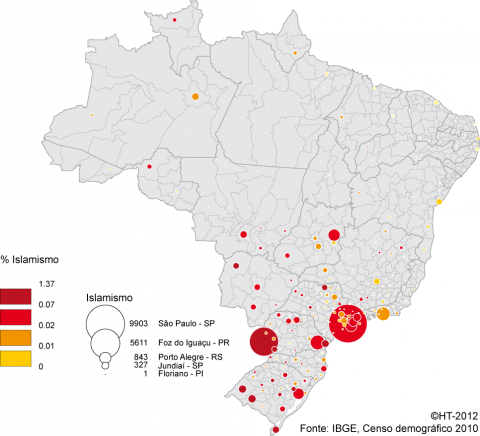
\includegraphics[width=.80\textwidth]{brasil_isla.png}
    % Caption centralizada
    \captionsetup[grafico]{justification=centering}
    % Fonte
    \captionfont{\small{\textbf{\\Fonte: Wikipedia}}}
    \end{figure}

\subsection{Localização:}
 Em todo o País, estima-se que existam oitenta centros do Islã e cerca de 50 mesquitas. As cidades de Foz do Iguaçu, Curitiba, Rio de Janeiro, Brasília e São Paulo abrigam as mais populosas comunidades de muçulmanos no Brasil. Notavelmente, na já citada Foz do Iguaçu, encontra-se o maior número de adeptos da religião. Além da presença de salas destinadas à oração e templos por quase todos os outros Estados que compõem a nação, em São Paulo há aproximadamente 10 mesquitas, sendo que a mais antiga é a Mesquita Brasil, fundada no continente latino-americano a partir do ano de 1929.

\section{O Islã no Mundo}
 \subsection{Adeptos:}
 A análise conduzida pelo centro de pesquisa trouxe dados interessantes. Há hoje no mundo 1,6 bilhão de pessoas que se designam muçulmanas.
 \subsection{Localização:}
 Embora o senso comum considere que a maioria dos seguidores dessa religião estejam no norte da África ou no Oriente Médio, apenas 20% deles encontram-se nesses lugares. A maioria dos muçulmanos (62%) está na região Ásia-Pacífico. O maior país muçulmano é a Indonésia. Pelo menos nos dias atuais: em 2050, calcula o estudo, o país com a maior comunidade islâmica do mundo será a Índia, que hoje tem como maior grupo religioso o hindu.

 \begin{figure}[ht]
    % Alterar espaçamentos antes e depois do caption
    \setlength{\abovecaptionskip}{5pt}
    \setlength{\belowcaptionskip}{0pt}
    % Caption
    \caption[Numero de adeptos do Islã no Mundo]
        {Numero de adeptos do Islã no Mundo}
    \centering
    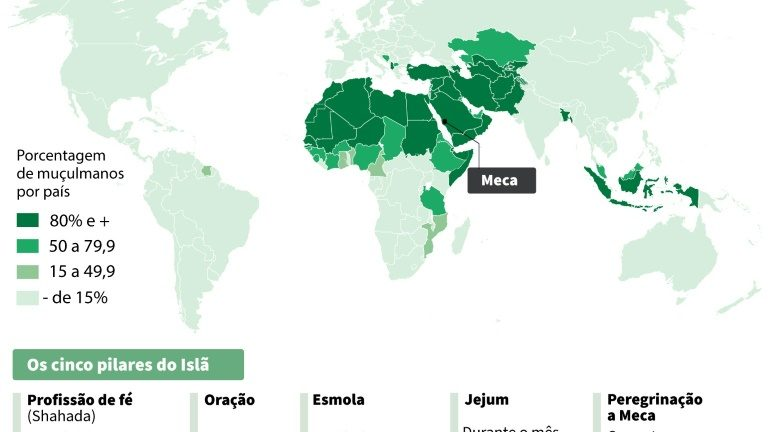
\includegraphics[width=1.10\textwidth]{mundo_isla.png}
    % Caption centralizada
    \captionsetup[grafico]{justification=centering}
    % Fonte
    \captionfont{\small{\textbf{\\Fonte: Wikipedia}}}
    \end{figure}

\end{document}